\subsection{Описание метода}

Предлагаемый метод инференса MoE моделей основан на переходе от жесткой коллективной схемы взаимодействия к клиент-серверной архитектуре. В коллективной схеме обмен активациями между рангами задается общей операцией All-to-All: все участники входят в заранее фиксированную группу и синхронно выполняют операции dispatch и combine. Такой подход хорошо согласуется с моделью статической раскладки экспертов по видеокартам, однако хуже подходит для сценариев, в которых нагрузка на экспертов меняется во время инференса, а клиентские экспертные блоки могут добавляться, исключаться или временно становиться недоступными.

В предлагаемой архитектуре MoE слой разделяется на сервер-оркестратор и набор удаленных экспертных блоков. Сервером является компонент \texttt{DistMoEBlock}: он выполняет роутинг, формирует задания dispatch, выбирает физический экспертный блок для обработки, управляет своими буферами обмена и выполняет операцию combine после получения результата. Клиентскую часть реализует компонент \texttt{DistExpertsBlock}. Он хранит локальное подмножество экспертов и выполняет вычислительные задания, поступающие от серверов-оркестраторов.

Различие между коллективной схемой и предлагаемой архитектурой удобно рассмотреть на одном цикле dispatch/combine. В коллективном подходе (рис.~\ref{fig:collective-moe-flow}) оба этапа выполняются всей группой участников. В предлагаемом методе (рис.~\ref{fig:dist-moe-flow}) dispatch выражается как адресное задание выбранному экспертному блоку, а combine выполняется тем же сервером-оркестратором после получения результата от клиента.

\begin{figure}[ht!]
    \centering
    \resizebox{0.64\textwidth}{!}{%
    \begin{tikzpicture}[
        component/.style={draw, rounded corners, align=center, minimum width=2.7cm, minimum height=0.9cm, fill=gray!8, font=\small},
        collective/.style={draw, rounded corners, align=center, minimum width=3.1cm, minimum height=0.8cm, fill=blue!8, font=\small},
        arrow/.style={->, thick},
        boundary/.style={->, thick, gray!70}
    ]
        \path[use as bounding box] (-1.55, -3.3) rectangle (8.55, 4.0);

        \node[component] (rank0) at (0, 3.1) {Ранг 0};
        \node[component] (rank1) at (3.5, 3.1) {Ранг 1};
        \node[component] (rank2) at (7.0, 3.1) {Ранг 2};

        \node[collective] (dispatch) at (3.5, 1.8) {dispatch\\All-to-All};

        \node[component] (expert0) at (0, 0.4) {Ранг 0};
        \node[component] (expert1) at (3.5, 0.4) {Ранг 1};
        \node[component] (expert2) at (7.0, 0.4) {Ранг 2};

        \node[collective] (combine) at (3.5, -1.0) {combine\\All-to-All};

        \node[component] (out0) at (0, -2.4) {Ранг 0};
        \node[component] (out1) at (3.5, -2.4) {Ранг 1};
        \node[component] (out2) at (7.0, -2.4) {Ранг 2};

        \draw[boundary] (0, 4.0) -- (rank0.north);
        \draw[boundary] (3.5, 4.0) -- (rank1.north);
        \draw[boundary] (7.0, 4.0) -- (rank2.north);

        \draw[arrow] (rank0) -- (dispatch);
        \draw[arrow] (rank1) -- (dispatch);
        \draw[arrow] (rank2) -- (dispatch);

        \draw[arrow] (dispatch) -- (expert0);
        \draw[arrow] (dispatch) -- (expert1);
        \draw[arrow] (dispatch) -- (expert2);

        \draw[arrow] (expert0) -- (combine);
        \draw[arrow] (expert1) -- (combine);
        \draw[arrow] (expert2) -- (combine);

        \draw[arrow] (combine) -- (out0);
        \draw[arrow] (combine) -- (out1);
        \draw[arrow] (combine) -- (out2);

        \draw[boundary] (out0.south) -- (0, -3.3);
        \draw[boundary] (out1.south) -- (3.5, -3.3);
        \draw[boundary] (out2.south) -- (7.0, -3.3);
    \end{tikzpicture}%
    }
    \caption{Один цикл dispatch/combine в коллективной схеме}
    \label{fig:collective-moe-flow}
\end{figure}

\begin{figure}[ht!]
    \centering
    \resizebox{0.64\textwidth}{!}{%
    \begin{tikzpicture}[
        server/.style={draw, rounded corners, align=center, minimum width=2.7cm, minimum height=0.9cm, fill=gray!8, font=\small},
        expert/.style={draw, rounded corners, align=center, minimum width=2.7cm, minimum height=0.9cm, fill=green!9, font=\small},
        exchange/.style={<->, thin, gray!70},
        boundary/.style={->, thick, gray!70},
        continuation/.style={->, semithick, gray!55}
    ]
        \path[use as bounding box] (-1.55, -0.6) rectangle (8.55, 4.0);

        \node[server] (s0) at (0, 3.1) {Ранг 0\\(сервер)};
        \node[server] (s1) at (3.5, 3.1) {Ранг 1\\(сервер)};
        \node[server] (s2) at (7.0, 3.1) {Ранг 2\\(сервер)};

        \node[expert] (e0) at (1.75, 0.1) {Экспертный\\блок 0\\(клиент)};
        \node[expert] (e1) at (5.25, 0.1) {Экспертный\\блок 1\\(клиент)};

        \draw[boundary] (0, 4.0) -- (s0.north);
        \draw[boundary] (3.5, 4.0) -- (s1.north);
        \draw[boundary] (7.0, 4.0) -- (s2.north);

        \draw[continuation] (s0.south) -- (0, -0.6);
        \draw[continuation] (s1.south) -- (3.5, -0.6);
        \draw[continuation] (s2.south) -- (7.0, -0.6);

        \draw[exchange] (s0) -- (e0);
        \draw[exchange] (s0) -- (e1);
        \draw[exchange] (s1) -- (e0);
        \draw[exchange] (s1) -- (e1);
        \draw[exchange] (s2) -- (e0);
        \draw[exchange] (s2) -- (e1);
    \end{tikzpicture}%
    }
    \caption{Один цикл dispatch/combine в предлагаемой архитектуре распределенного MoE слоя}
    \label{fig:dist-moe-flow}
\end{figure}

Ключевое следствие такого разделения состоит в том, что выбор исполнителя становится частью логики инференса, а не только следствием заранее заданной коллективной конфигурации. Если эксперт представлен несколькими физическими репликами, сервер-оркестратор может выбрать одну из них с учетом текущей доступности и очереди заданий. При этом клиентские части могут создаваться, удаляться или временно исключаться прямо во время работы системы: сервер обновляет пул доступных экспертных блоков и планирует последующие задания уже с учетом нового состава исполнителей.

Для передачи активаций и результатов вычислений между сервером и клиентами используется абстракция \texttt{TensorTransferEngine} (TTE). Она связывает управляющую часть MoE слоя с конкретным механизмом адресной передачи GPU-памяти. Управляющие сообщения передают метаданные задания, а сами активации и результаты размещаются в заранее зарегистрированных буферах, доступных для чтения и записи между удаленными устройствами.

Во время одного вызова MoE слоя сервер сначала вычисляет значения роутера и определяет top-\(k\) экспертов для входных активаций. Затем активации группируются по экспертам, для каждой порции создается задание обработки, выбирается экспертный блок и выполняется dispatch. Удаленный экспертный блок читает входные данные из серверного буфера, выполняет локальные экспертные вычисления, записывает результат в выходной буфер сервера и отправляет уведомление о завершении. После этого сервер выполняет combine: считывает готовую часть результата и добавляет ее в выходной батч слоя с учетом весов роутинга.

\subsection{Архитектура метода}

На рисунке~\ref{fig:method-class-diagram} показана общая структура предлагаемой архитектуры. Диаграмма отделяет серверную часть от клиентской и показывает только основные компоненты: оркестратор MoE слоя, пул экспертных блоков, задачи обработки, пулы буферов и экземпляры TTE на обеих сторонах взаимодействия.

\begin{figure}[ht!]
    \centering
    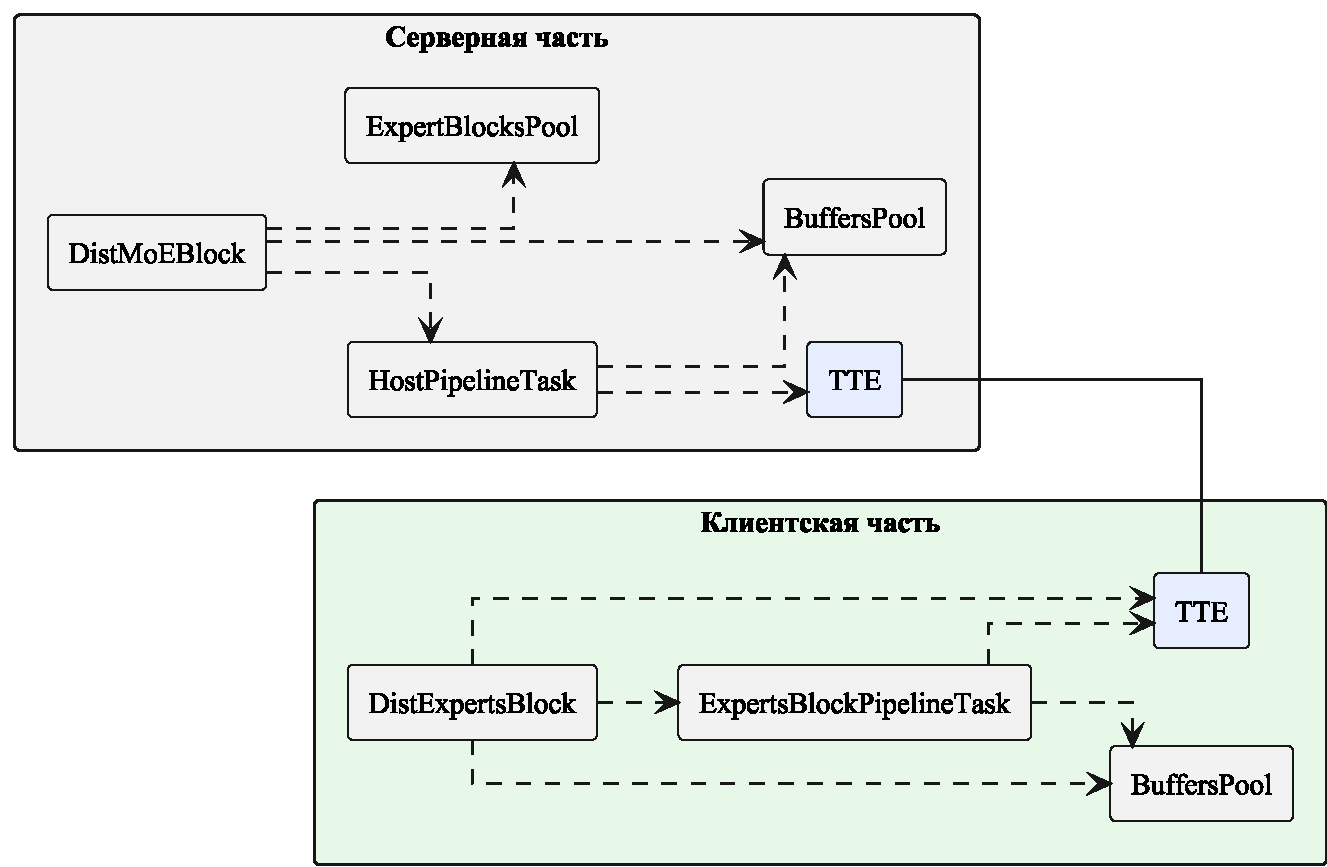
\includegraphics[width=0.86\textwidth]{diagrams/method-components.pdf}
    \caption{UML-диаграмма основных компонентов}
    \label{fig:method-class-diagram}
\end{figure}

В этой структуре управляющий контур (control plane) и контур передачи данных (data plane) разделены. Управляющий контур отвечает за выбор исполнителя, сериализацию метаданных и уведомления о состоянии задания. Контур передачи данных работает с зарегистрированными областями памяти: экспертные активации читаются экспертным блоком из зарезервированного серверного буфера, а результат вычислений записывается обратно в выходной буфер, зарезервированный на сервере для данного dispatch.

Диаграмма последовательности одного цикла dispatch/combine приведена на рисунке~\ref{fig:method-sequence-diagram}. Она фиксирует порядок операций на уровне программных компонентов: подготовку метаданных по экспертам, создание конвейерной задачи, выбор экспертного блока, отправку управляющего сообщения \texttt{DispatchSubmit}, создание клиентской задачи, чтение данных с сервера, экспертные вычисления, запись результата и обратное уведомление о готовности выходного буфера, после которого запускается операция combine.

\begin{figure}[ht!]
    \centering
    \makebox[\textwidth][c]{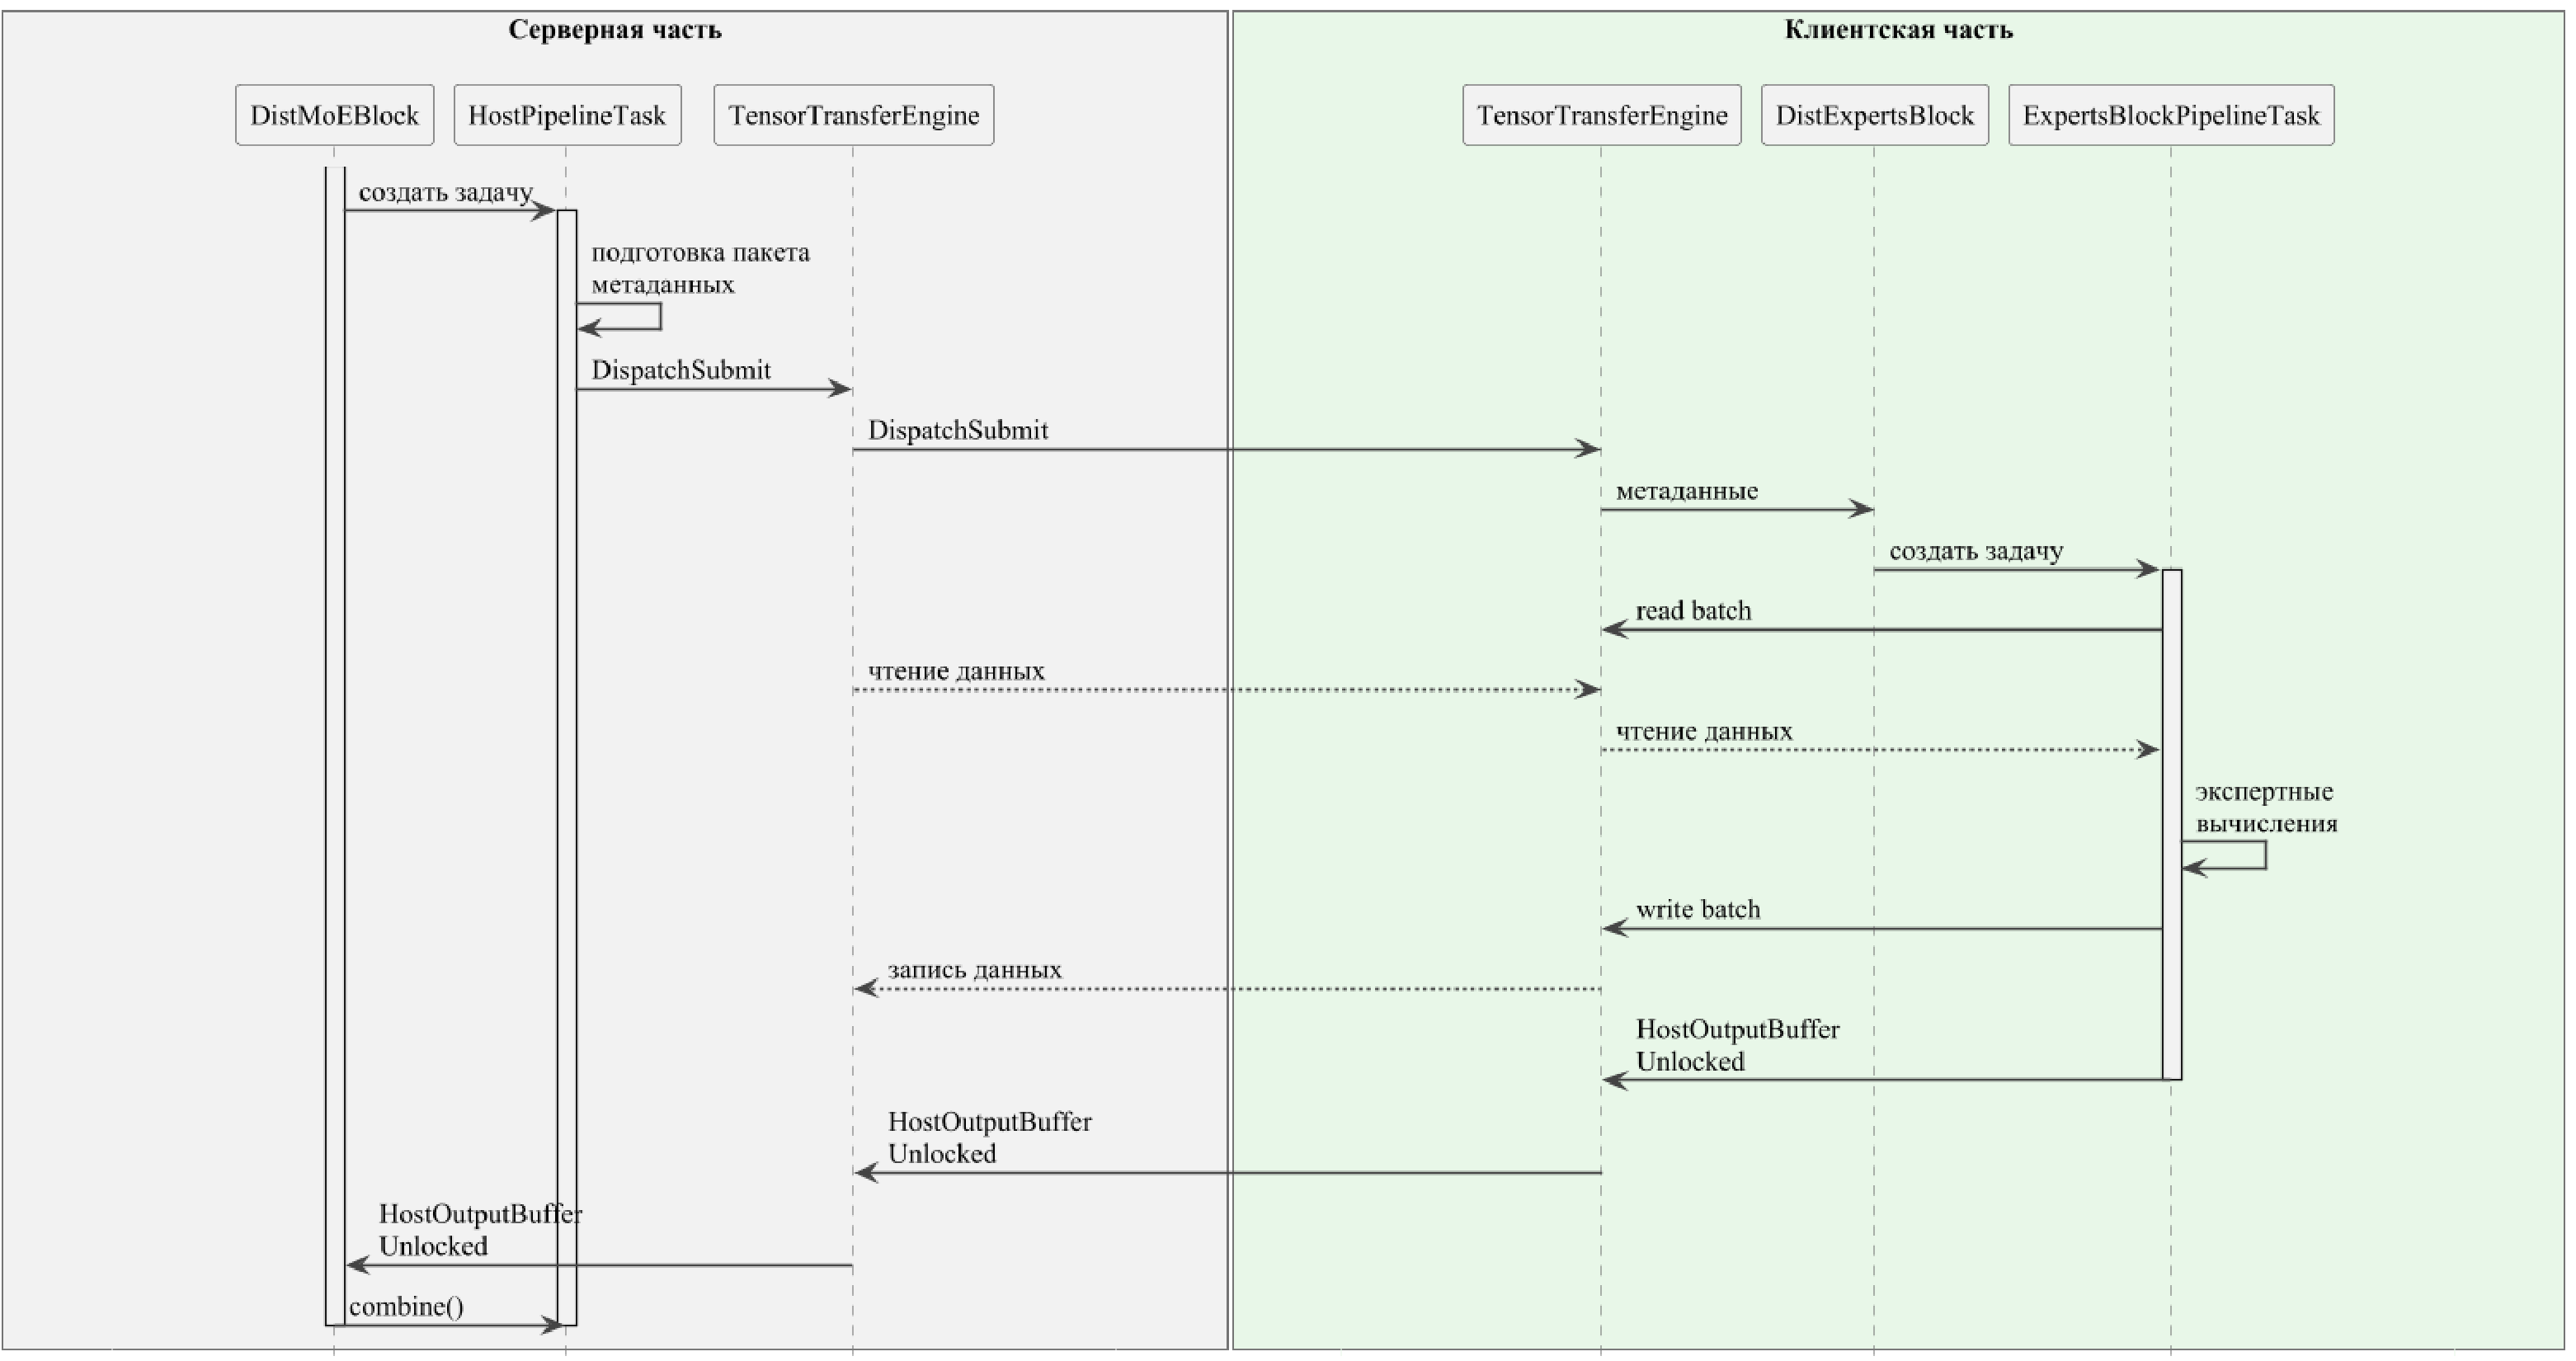
\includegraphics[width=1.12\textwidth]{diagrams/method-sequence.pdf}}
    \caption{UML-диаграмма последовательности одного цикла dispatch/combine}
    \label{fig:method-sequence-diagram}
\end{figure}

Пулы буферов используются на обеих сторонах взаимодействия. На сервере они ограничивают число одновременно выполняемых передач и связывают каждое задание с конкретным входным и выходным буфером. На клиенте они позволяют переиспользовать локальные области памяти для чтения входных данных и записи результата. Такое устройство передаваемой памяти дает возможность организовать конвейерное выполнение: пока один буфер используется для экспертных вычислений, другой может участвовать в чтении следующей порции активаций или записи уже готового результата. За счет этого операции чтения и записи могут перекрываться с вычислениями, а канал передачи данных и шина памяти используются более эффективно, что будет показано в экспериментах.

\subsection{Компонент \texttt{DistMoEBlock}}

Компонент \texttt{DistMoEBlock} реализует серверную часть распределенного MoE слоя. Его ответственность состоит в оркестрации всего распределенного MoE слоя: подготовить входной батч к обработке экспертами, распределить работу по удаленным блокам, принять готовые результаты и агрегировать их в выходной батч слоя.

\begin{figure}[ht!]
    \centering
    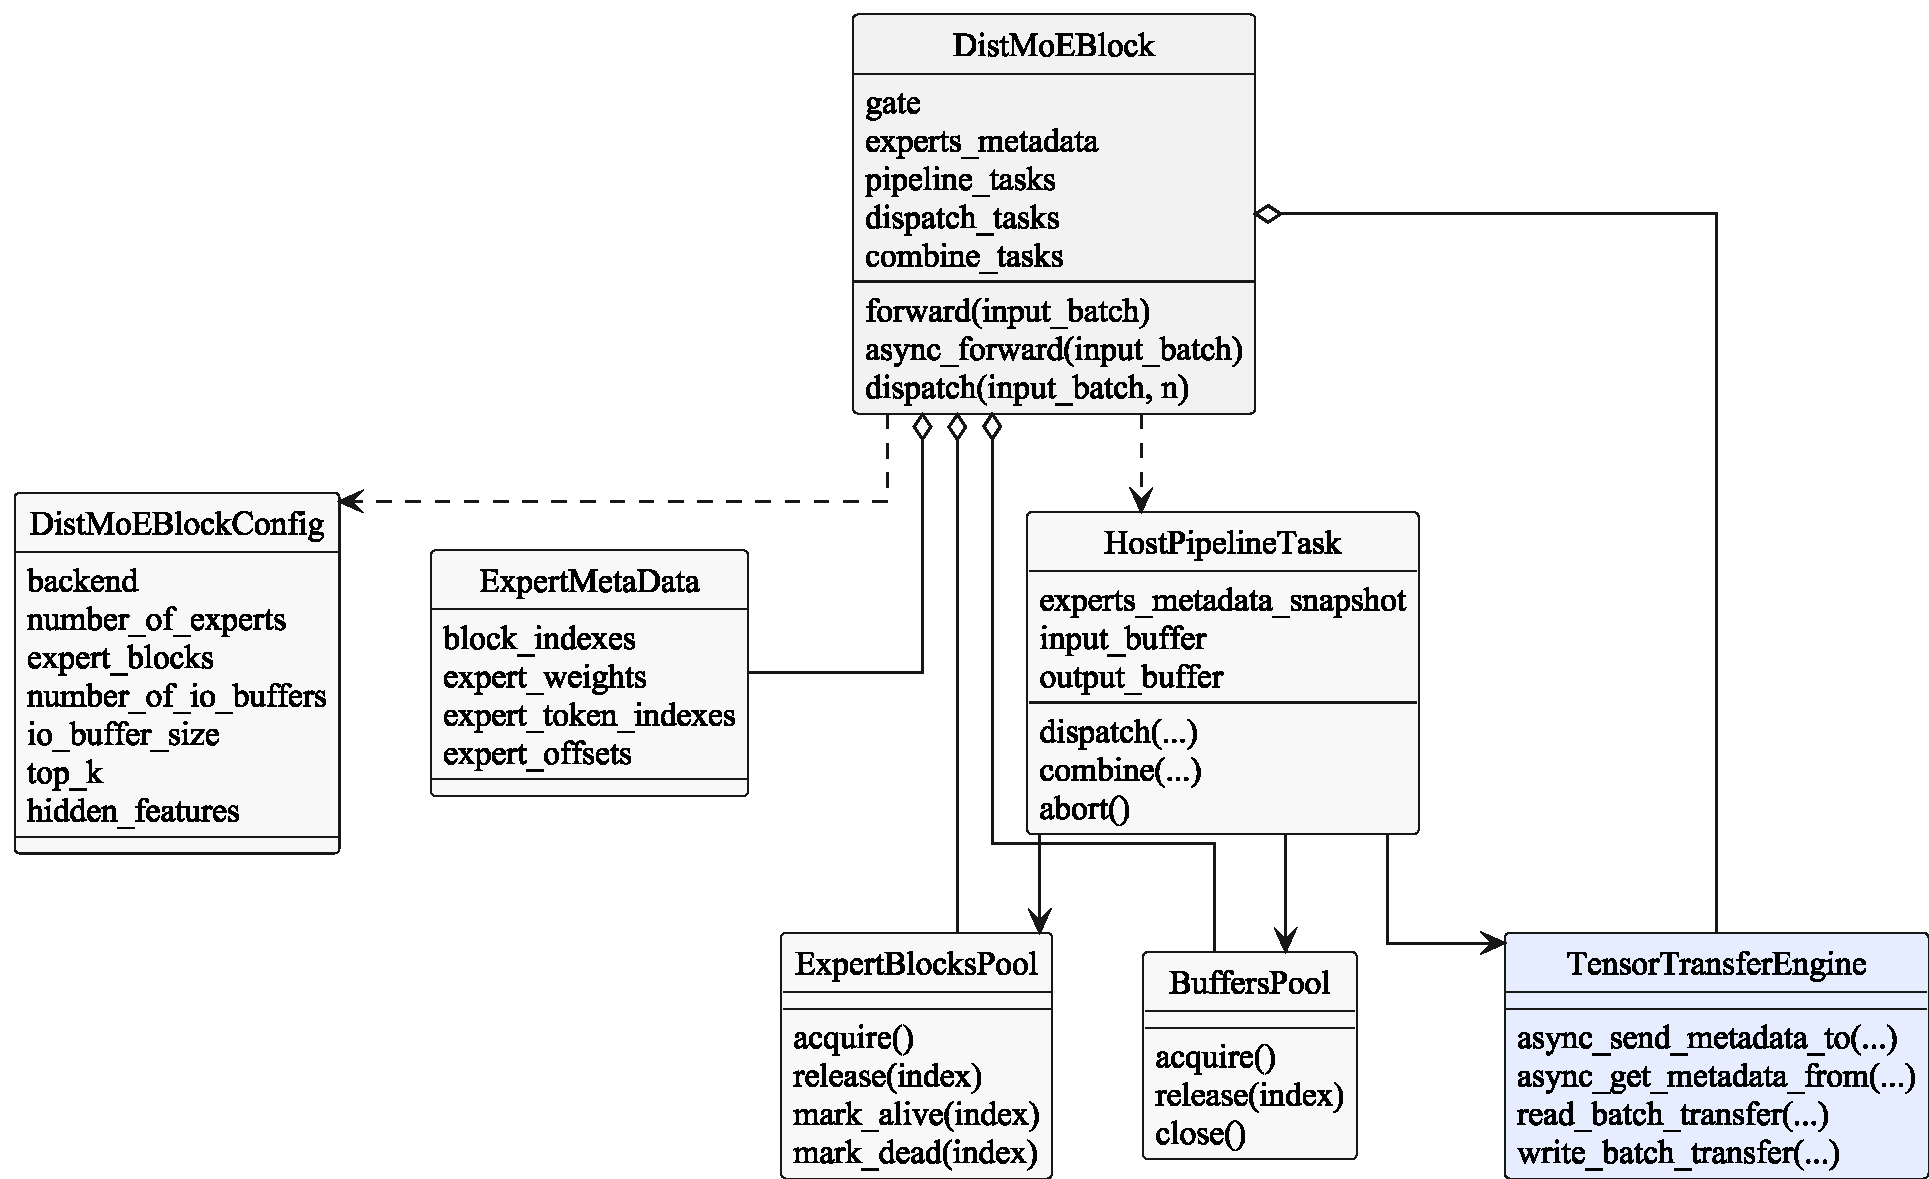
\includegraphics[width=\textwidth]{diagrams/distmoe-class.pdf}
    \caption{UML-диаграмма классов серверной части \texttt{DistMoEBlock}}
    \label{fig:distmoe-class-diagram}
\end{figure}

На рисунке~\ref{fig:distmoe-class-diagram} показаны основные связи серверной части. \texttt{DistMoEBlock} содержит роутер \texttt{gate}, метаданные экспертов, пул доступных экспертных блоков, два пула буферов и серверный экземпляр TTE. Сначала роутер вычисляет веса и индексы top-\(k\) экспертов. Для каждого выбранного эксперта компонент хранит индексы токенов, веса роутинга и очередь еще не обработанных отрезков активаций.

Dispatch на серверной стороне выполняется через \texttt{HostPipelineTask}. Задача выбирает экспертный блок из \texttt{ExpertBlocksPool}, формирует пакет метаданных по экспертам, резервирует входной и выходной буферы на стороне сервера, копирует нужные активации в зарезервированный входной буфер и отправляет управляющее сообщение \texttt{DispatchSubmit}. При подтверждении готовности результата сервер вызывает combine для соответствующей задачи: данные из выходного буфера добавляются в общий выходной батч с учетом весов роутинга.

Отдельная часть ответственности \texttt{DistMoEBlock} связана с динамическим состоянием экспертных блоков. Компонент поддерживает фоновые проверки доступности, умеет помечать блоки как доступные или недоступные и отменять незавершенные задания, отправленные на блок, ставший недоступным. При отмене задания его отрезки активаций возвращаются в очереди обработки, поэтому дальнейший dispatch может быть направлен на другой доступный экспертный блок с нужными экспертами. Эти служебные механизмы на диаграмме не детализированы, чтобы сохранить фокус на основных компонентах серверной части.

\subsection{Компонент \texttt{DistExpertsBlock}}

Компонент \texttt{DistExpertsBlock} реализует клиентскую часть архитектуры. Его задача состоит в том, чтобы принять задание от сервера, выполнить локальные экспертные вычисления, записать полученный результат в серверный буфер и сообщить серверу о завершении задачи.

\begin{figure}[ht!]
    \centering
    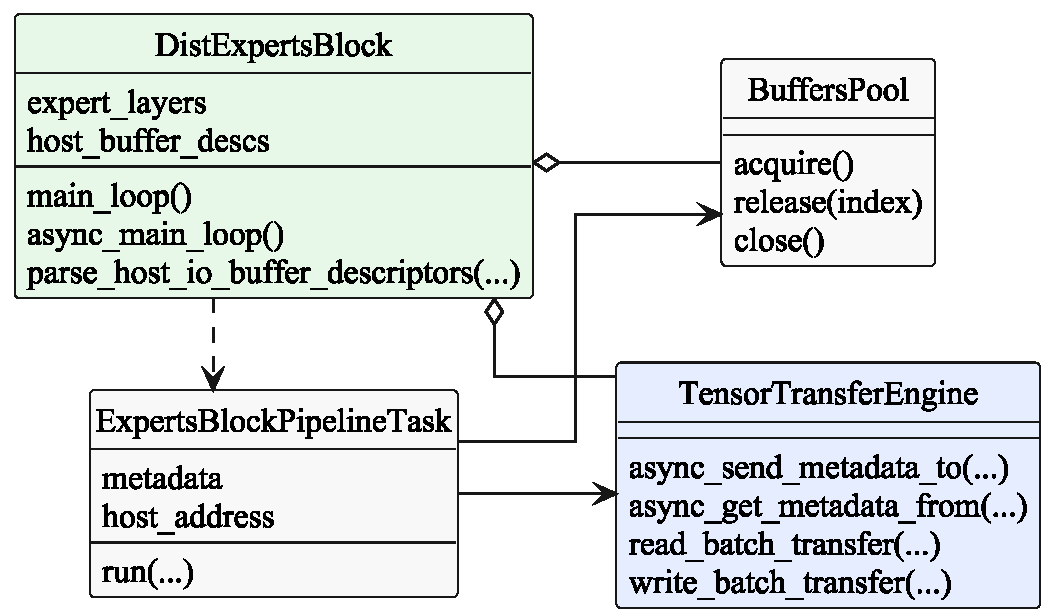
\includegraphics[width=0.546\textwidth]{diagrams/distexperts-class.pdf}
    \caption{UML-диаграмма классов клиентской части \texttt{DistExpertsBlock}}
    \label{fig:distexperts-class-diagram}
\end{figure}

На рисунке~\ref{fig:distexperts-class-diagram} приведена структура клиентской части. Компонент хранит локальные экспертные слои, пулы локальных входных и выходных буферов, а также дескрипторы серверных буферов, полученные во время инициализации. Основной цикл компонента принимает управляющие сообщения от сервера: сообщение с дескрипторами серверных буферов обновляет локальные таблицы, а сообщение \texttt{DispatchSubmit} приводит к созданию клиентской задачи обработки.

\texttt{ExpertsBlockPipelineTask} разбирает метаданные задания, получает дескрипторы серверных буферов и резервирует локальные буферы. Затем задача выполняет чтение входного батча через TTE, запускает локальные экспертные вычисления и записывает результат обратно в серверный выходной буфер. После успешной записи клиент отправляет серверу уведомление \texttt{HostOutputBufferUnlocked}; это уведомление означает, что серверный выходной буфер содержит готовую часть результата и может быть использован на этапе combine.

Вычислительная часть поддерживает два режима. Если доступен grouped GeMM и он разрешен для задания, вычисления по нескольким экспертам выполняются через групповую матричную операцию. В противном случае используется последовательный проход по экспертам внутри блока. Оба режима сохраняют одну и ту же внешнюю семантику: клиент получает входные активации, применяет соответствующие экспертные слои и записывает выход в буфер, указанный сервером.

\subsection{Компонент \texttt{TensorTransferEngine}}

\texttt{TensorTransferEngine} является связующей компонентой распределенного MoE слоя. В архитектуре существует отдельный экземпляр TTE на стороне сервера и отдельные экземпляры на стороне клиентских блоков; они обмениваются управляющими сообщениями и выполняют адресные операции чтения и записи между зарегистрированными областями памяти.

\begin{figure}[ht!]
    \centering
    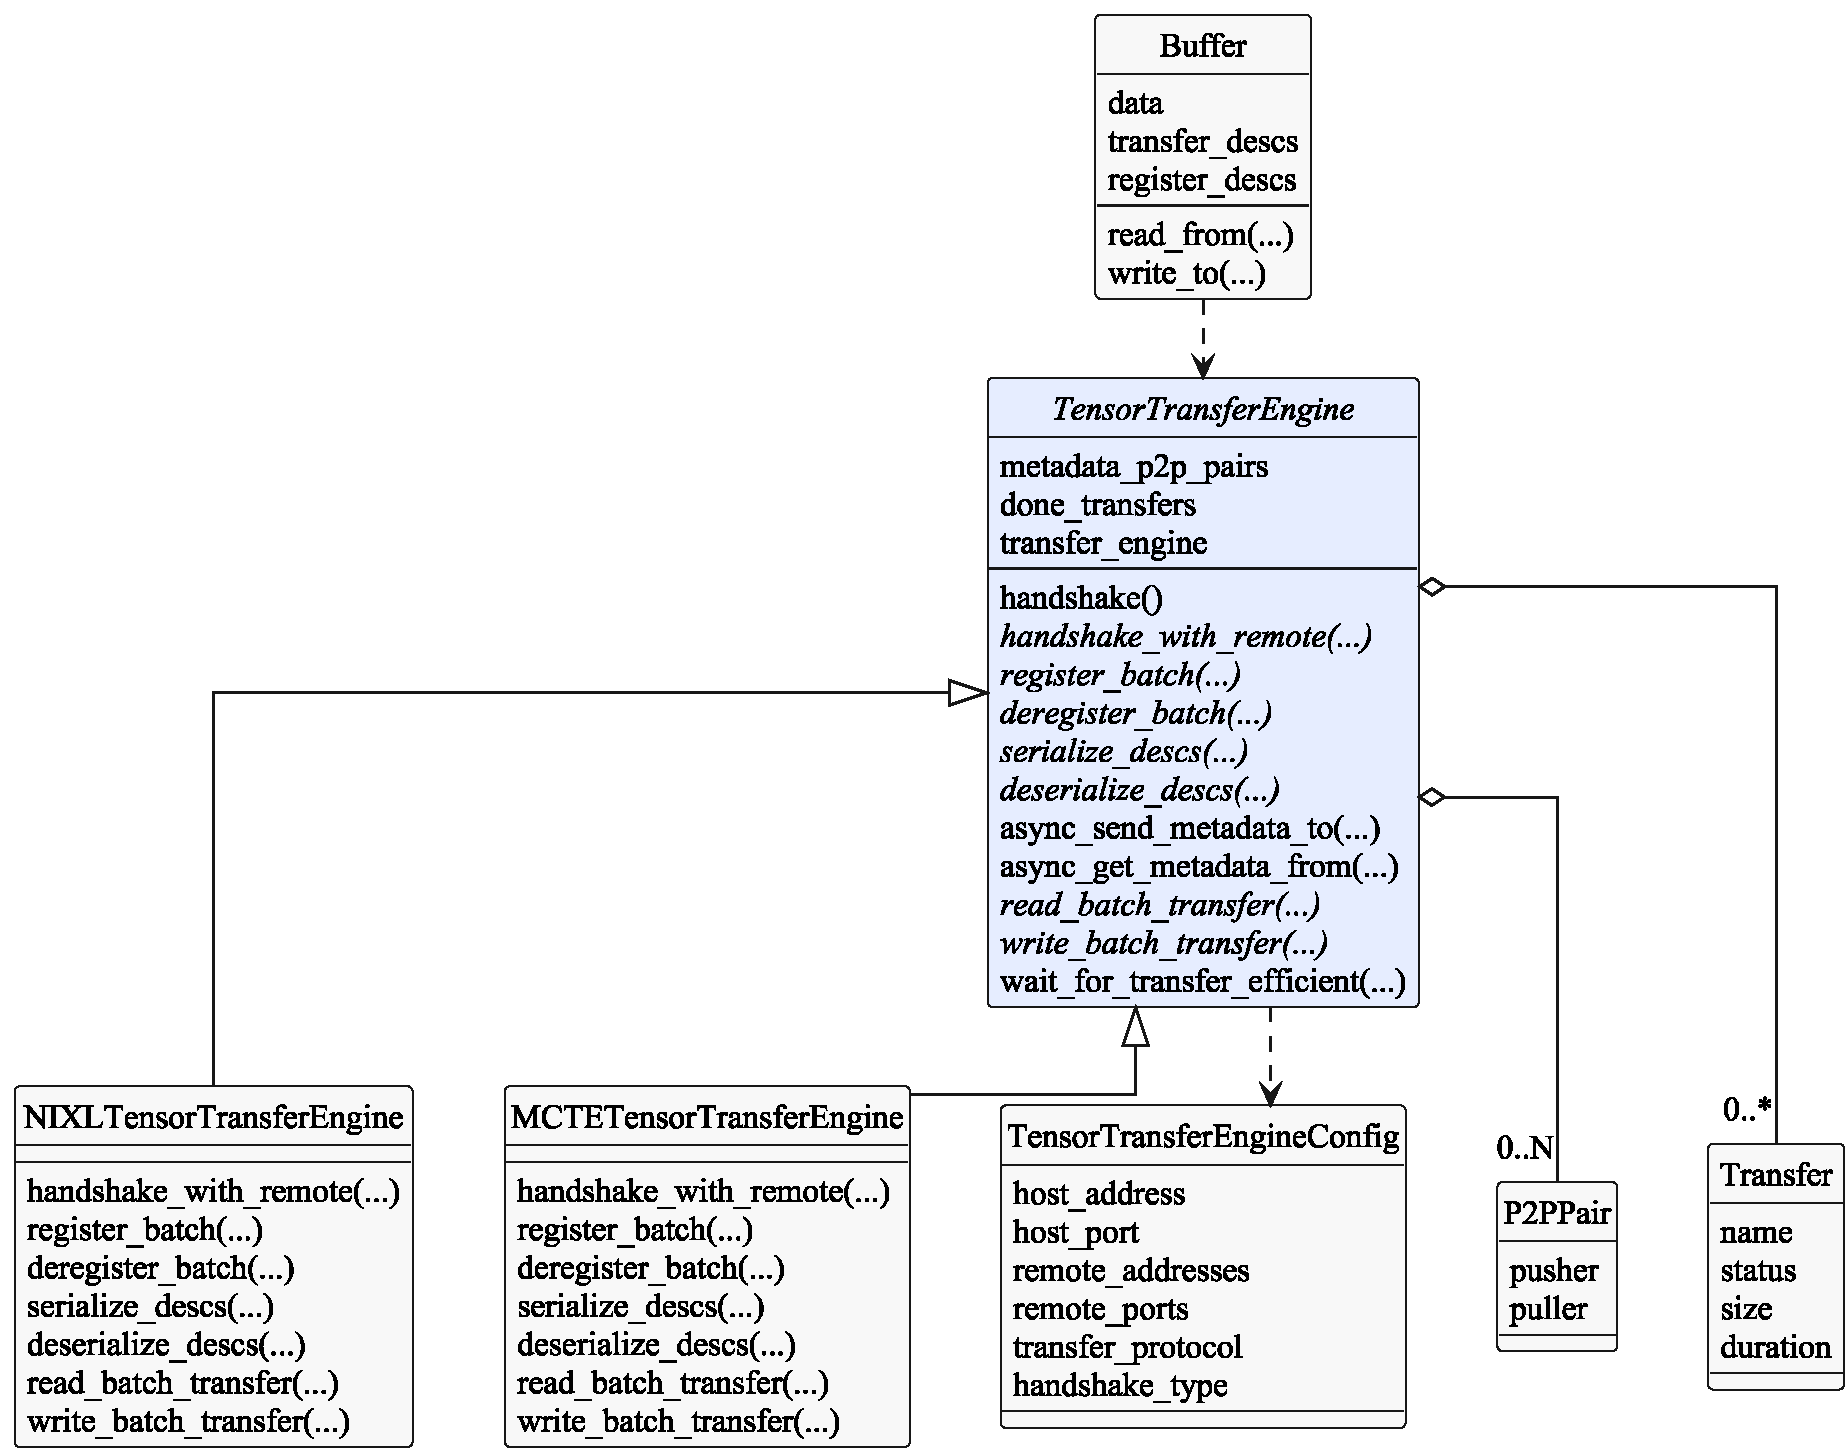
\includegraphics[width=0.957\textwidth]{diagrams/tte-class.pdf}
    \caption{UML-диаграмма классов компонента \texttt{TensorTransferEngine}}
    \label{fig:tte-class-diagram}
\end{figure}

На рисунке~\ref{fig:tte-class-diagram} показано место TTE в реализации передачи данных. Базовый класс задает общий интерфейс для регистрации и снятия регистрации памяти, сериализации и десериализации дескрипторов, отправки и приема управляющих сообщений, запуска операций чтения и записи, а также ожидания завершения асинхронных передач. Реализации на основе NIXL и MCTE используют этот интерфейс для подключения движков адресной передачи данных.

Буфер в этой архитектуре является зарегистрированной областью памяти на конкретном устройстве. При создании буфера TTE регистрирует его данные, получает дескрипторы передачи и сериализует их для передачи на экспертные блоки. Поэтому серверная и клиентская задачи работают не с низкоуровневыми деталями конкретного движка, а абстракциями более высокого уровня: буферами и их дескрипторами.

Фоновый мониторинг передач внутри TTE отслеживает состояние запущенных операций и позволяет задачам ожидать завершения конкретного чтения или записи. Это важно для корректного конвейера операций dispatch/combine: экспертные вычисления должны начинаться только после завершения чтения входного батча, а уведомление \texttt{HostOutputBufferUnlocked} должно отправляться только после завершения записи результата в серверный буфер.

\clearpage

\subsection*{Выводы по главе}
\addcontentsline{toc}{subsection}{Выводы по главе}

В главе представлен метод, в котором MoE слой разделяется на оркестратор и набор удаленных экспертных блоков. Оркестратор (сервер) принимает решения о роутинге, выборе исполнителей, постановке заданий и объединении результатов, а экспертные блоки (клиенты) выполняют локальные вычисления над переданными активациями.

Ключевое отличие предложенного подхода от коллективной схемы состоит в том, что обработка активаций выражается через адресные задания конкретным вычислительным модулям. Это создает основу для динамической балансировки нагрузки, повторного выбора физической реплики эксперта и продолжения инференса при недоступности части экспертных блоков.
